\documentclass[a4paper]{article}

% matematyka
\usepackage{amsmath, amssymb, graphics, setspace}

% odpowiednie kodowanie
\usepackage[utf8]{inputenc}
\usepackage[T1]{fontenc}

% dodatkowa czcionka
\usepackage{times}

% polskie parametry tekstu
\usepackage[polish]{babel}

% grafika
\usepackage{graphicx}

% kolory
\usepackage{xcolor}

% tabele
\usepackage{dcolumn}

% kodowanie
% https://en.wikibooks.org/wiki/LaTeX/Source_Code_Listings
\usepackage{listings}
\lstset{
   numbers=left,
   tabsize=3,
   numberstyle=\footnotesize,
   basicstyle=\ttfamily \footnotesize \color{black},
   breaklines=true,
   escapeinside={(*@}{@*)}
 }



% dodatkowe definicje
\newcommand{\mathsym}[1]{{}}
\newcommand{\unicode}[1]{{}}


\begin{document}

\title{Raport: Organizacja projektu badawczego}
\author{Michał Gawryluk}
\date{\today}
\maketitle


% --- Wprowadzenie --------------------------
\section{Wprowadzenie}

Celem raportu jest wykorzystanie metod poznanych na przedmiocie "Organizacja projektu badawczego" i ukazanie wszystkich narzędzi git,LaTeX, cmake, języka programistycznego do automatycznego generowania pracy badawczej.
Do raportu został użyty zbiór danych o przestępczości w USA per stan. R został wybrany, jako główny język programistyczny do analityki.

Wykres populacji z przestępczością o charakterze napaści został zaprezentowany poniżej. Każdy punkt reprezentowany jest przez jeden stan.

\begin{figure}[hbt]
  \centering
  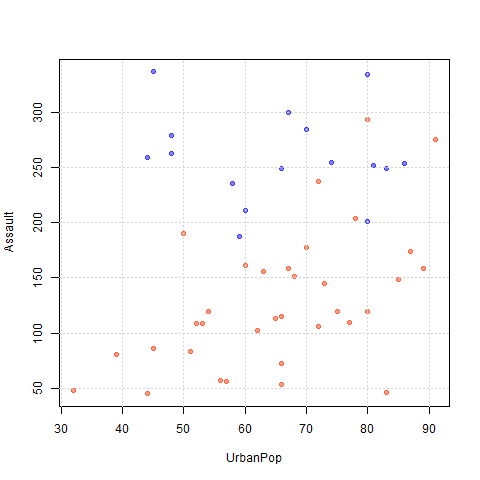
\includegraphics[width = .65\textwidth]{./analiza/analiza_mg_fig_1}
  \caption{Zależność ceny od przebiegu}
\end{figure}

Całość danych użytych do raportu została zaprezentowana w Tablica 1.


% Table created by stargazer v.5.2.2 by Marek Hlavac, Harvard University. E-mail: hlavac at fas.harvard.edu
% Date and time: wt., cze 16, 2020 - 20:02:37
% Requires LaTeX packages: dcolumn 
\begin{table}[!htbp] \centering 
  \caption{Podstawowe statystyki dla wykorzystanych danych} 
  \label{tab:analiza_mg_tab_1} 
\small 
\begin{tabular}{@{\extracolsep{5pt}} D{.}{.}{-3} D{.}{.}{-3} D{.}{.}{-3} D{.}{.}{-3} } 
\\[-1.8ex]\hline 
\hline \\[-1.8ex] 
\multicolumn{1}{c}{} & \multicolumn{1}{c}{Murder} & \multicolumn{1}{c}{Assault} & \multicolumn{1}{c}{UrbanPop} \\ 
\hline \\[-1.8ex] 
\multicolumn{1}{c}{1} & 13.200 & 236 & 58 \\ 
\multicolumn{1}{c}{2} & 10 & 263 & 48 \\ 
\multicolumn{1}{c}{3} & 8.100 & 294 & 80 \\ 
\multicolumn{1}{c}{4} & 8.800 & 190 & 50 \\ 
\multicolumn{1}{c}{5} & 9 & 276 & 91 \\ 
\multicolumn{1}{c}{6} & 7.900 & 204 & 78 \\ 
\multicolumn{1}{c}{7} & 3.300 & 110 & 77 \\ 
\multicolumn{1}{c}{8} & 5.900 & 238 & 72 \\ 
\multicolumn{1}{c}{9} & 15.400 & 335 & 80 \\ 
\multicolumn{1}{c}{10} & 17.400 & 211 & 60 \\ 
\multicolumn{1}{c}{11} & 5.300 & 46 & 83 \\ 
\multicolumn{1}{c}{12} & 2.600 & 120 & 54 \\ 
\multicolumn{1}{c}{13} & 10.400 & 249 & 83 \\ 
\multicolumn{1}{c}{14} & 7.200 & 113 & 65 \\ 
\multicolumn{1}{c}{15} & 2.200 & 56 & 57 \\ 
\multicolumn{1}{c}{16} & 6 & 115 & 66 \\ 
\multicolumn{1}{c}{17} & 9.700 & 109 & 52 \\ 
\multicolumn{1}{c}{18} & 15.400 & 249 & 66 \\ 
\multicolumn{1}{c}{19} & 2.100 & 83 & 51 \\ 
\multicolumn{1}{c}{20} & 11.300 & 300 & 67 \\ 
\multicolumn{1}{c}{21} & 4.400 & 149 & 85 \\ 
\multicolumn{1}{c}{22} & 12.100 & 255 & 74 \\ 
\multicolumn{1}{c}{23} & 2.700 & 72 & 66 \\ 
\multicolumn{1}{c}{24} & 16.100 & 259 & 44 \\ 
\multicolumn{1}{c}{25} & 9 & 178 & 70 \\ 
\multicolumn{1}{c}{26} & 6 & 109 & 53 \\ 
\multicolumn{1}{c}{27} & 4.300 & 102 & 62 \\ 
\multicolumn{1}{c}{28} & 12.200 & 252 & 81 \\ 
\multicolumn{1}{c}{29} & 2.100 & 57 & 56 \\ 
\multicolumn{1}{c}{30} & 7.400 & 159 & 89 \\ 
\multicolumn{1}{c}{31} & 11.400 & 285 & 70 \\ 
\multicolumn{1}{c}{32} & 11.100 & 254 & 86 \\ 
\multicolumn{1}{c}{33} & 13 & 337 & 45 \\ 
\multicolumn{1}{c}{34} & 0.800 & 45 & 44 \\ 
\multicolumn{1}{c}{35} & 7.300 & 120 & 75 \\ 
\multicolumn{1}{c}{36} & 6.600 & 151 & 68 \\ 
\multicolumn{1}{c}{37} & 4.900 & 159 & 67 \\ 
\multicolumn{1}{c}{38} & 6.300 & 106 & 72 \\ 
\multicolumn{1}{c}{39} & 3.400 & 174 & 87 \\ 
\multicolumn{1}{c}{40} & 14.400 & 279 & 48 \\ 
\multicolumn{1}{c}{41} & 3.800 & 86 & 45 \\ 
\multicolumn{1}{c}{42} & 13.200 & 188 & 59 \\ 
\multicolumn{1}{c}{43} & 12.700 & 201 & 80 \\ 
\multicolumn{1}{c}{44} & 3.200 & 120 & 80 \\ 
\multicolumn{1}{c}{45} & 2.200 & 48 & 32 \\ 
\multicolumn{1}{c}{46} & 8.500 & 156 & 63 \\ 
\multicolumn{1}{c}{47} & 4 & 145 & 73 \\ 
\multicolumn{1}{c}{48} & 5.700 & 81 & 39 \\ 
\multicolumn{1}{c}{49} & 2.600 & 53 & 66 \\ 
\multicolumn{1}{c}{50} & 6.800 & 161 & 60 \\ 
\hline \\[-1.8ex] 
\end{tabular} 
\end{table} 


W całym zbiorze średnia liczba napaści wynosi \(170.76\)
 a średni liczba mordersw to \(7.79\)
.
 
\pagebreak 
 
\section{Kod}

Kod pierwszego rozwiązania oparty jest o następujące pakiety.

\lstinputlisting[language=R, linerange={1-3}, caption=Wykorzystanie pakiety (zawarte w pliku \lstname)]{./analiza/analiza_mg.R}

Fragment tworzący automatyczne wartości. 

\lstinputlisting[linerange={23-36}, caption=Tworzenie tablicy (zawarte w pliku \lstname)]{./analiza/analiza_mg.R}



\end{document}
%%% Local Variables:
%%% mode: latex
%%% TeX-master: t
%%% End:
